\section{Introduction}
\lblsec{intro}






\begin{figure}
    \centering
    \vspace{-0.5cm}%
    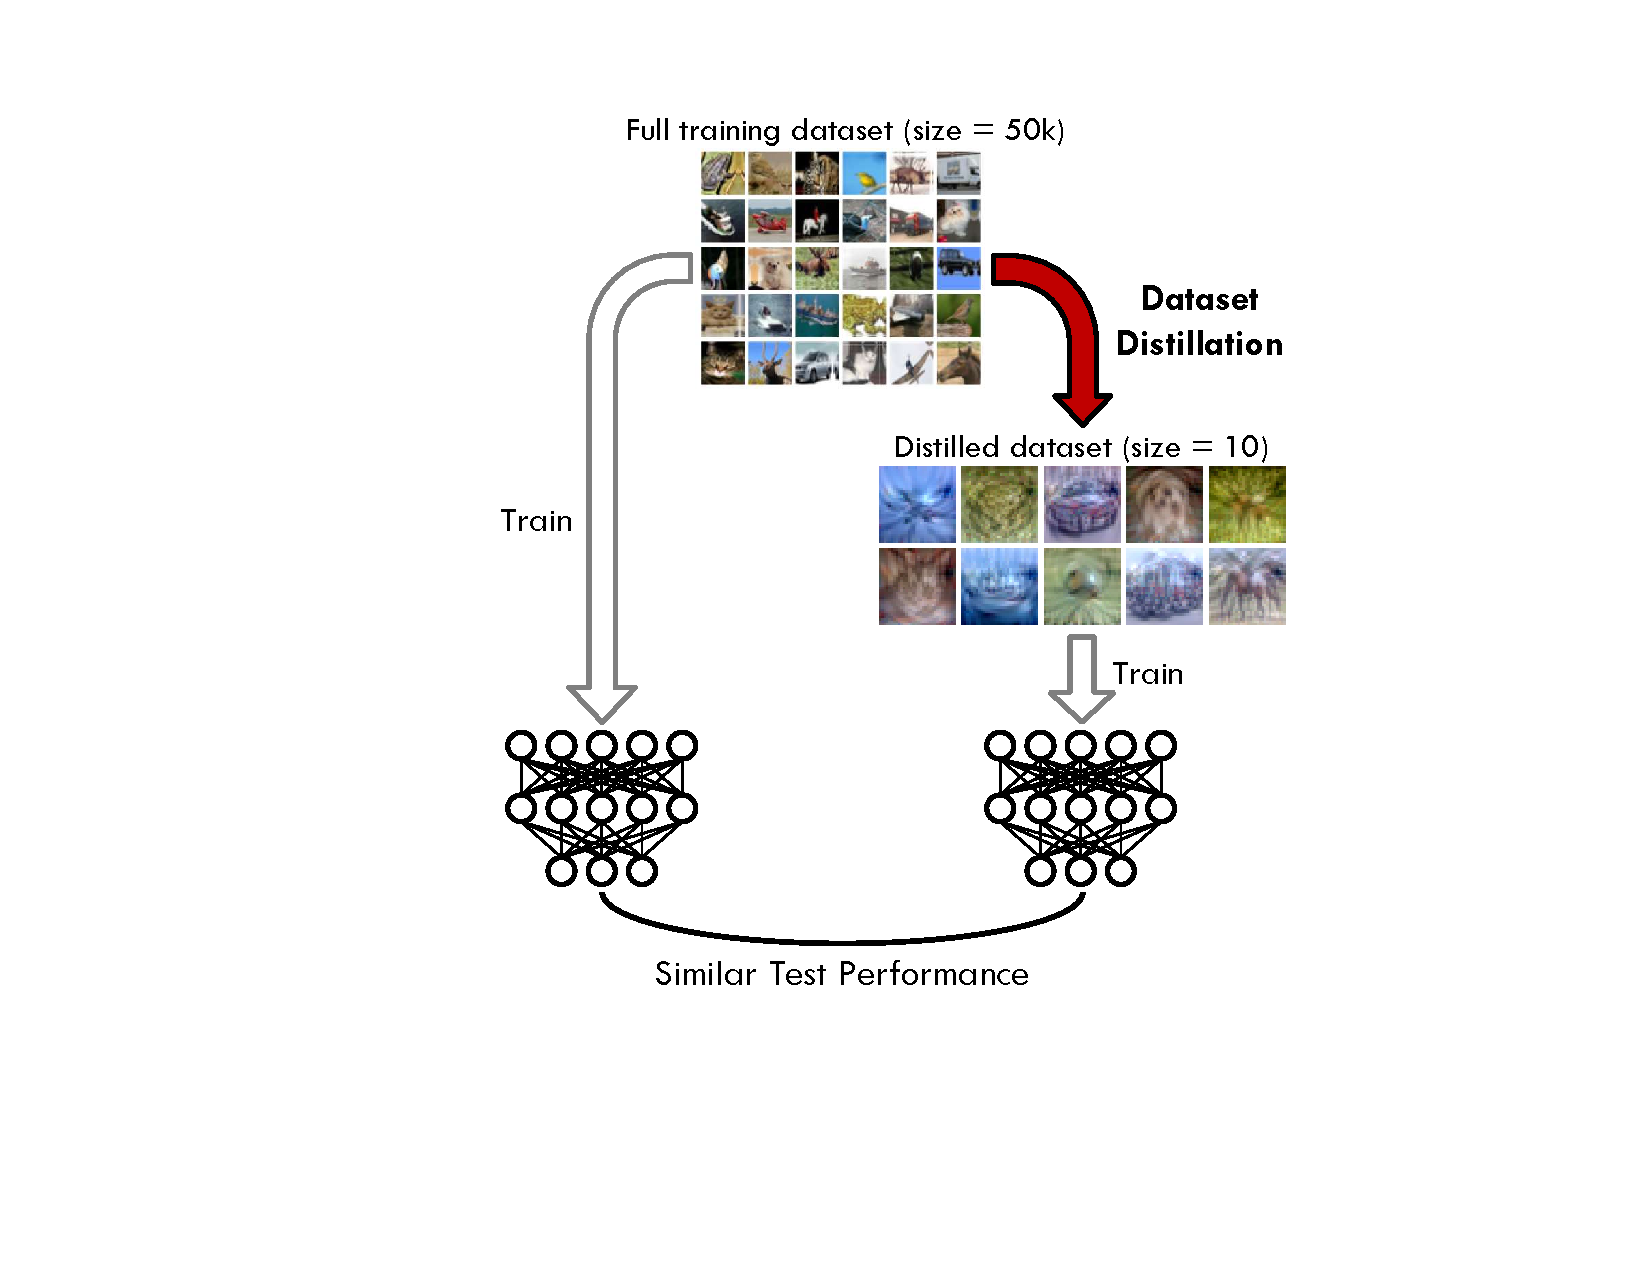
\includegraphics[scale=0.58, trim=230 106 150 20, clip]{figures/figure_2_dataset_distillation.pdf}\vspace{-0.85cm}
    \caption{Dataset distillation aims to generate a small synthetic dataset for which a model trained on it can achieve a similar test performance as a model trained on the whole real train set.}%
    \lblfig{dataset_distillation}\vspace{-5pt}
\end{figure}

In the seminal 2015 paper, Hinton et al.~\cite{hinton2015distilling} proposed {\em model distillation}, which aims to distill the knowledge of a complex model into a simpler one.  
{\em Dataset distillation}, proposed by Wang et al.~\cite{dd}, is a related but orthogonal task: rather
than distilling the model, the idea is to distill the dataset. 
As shown in Figure~\ref{fig:dataset_distillation}, the goal is to distill the knowledge from a large training dataset into a very small set of synthetic training images (as low as one image per class) such that training a model on the distilled data would give a similar test performance as training one on the original dataset. Dataset distillation has become a lively research topic in machine learning~\cite{bohdal2020flexible,sucholutsky2021soft,dc,dsa,nguyen2020dataset,nguyen2021dataset,dm} with various applications, such as continual learning, neural architecture search, and privacy-preserving ML. Still, the problem has so far been of mainly theoretical interest, since most prior methods focus on toy datasets, like MNIST and \mbox{CIFAR}, while struggling on real, higher-resolution images. In this work, we present a new approach to dataset distillation that not only outperforms previous work in performance, but is also applicable to large-scale datasets, as shown in \reffig{teaser}.


Unlike classical data compression, dataset distillation aims for a small synthetic dataset that still retains adequate task-related information so that models trained on it can generalize to unseen test data, as shown in \reffig{dataset_distillation}. Thus, the distilling algorithm must strike a delicate balance by heavily compressing information without completely obliterating the discriminative features.  
To do this, dataset distillation methods attempt to discover exactly which aspects of the real data are critical for learning said discrimination. Several methods consider end-to-end training~\cite{dd,nguyen2020dataset,nguyen2021dataset} but often require huge compute and memory and suffer from inexact relaxation~\cite{nguyen2020dataset,nguyen2021dataset} or training instability of unrolling many iterations~\cite{dd,maclaurin2015gradient}. To reduce the optimization difficulty, other methods~\cite{dc,dsa} focus on short-range behavior, enforcing a single training step on distilled data to match that on real data. However, error may accumulate in evaluation, where the distilled data is applied over many steps. We confirm this hypothesis experimentally in \refsec{shortlongrange}.


To address the above challenges, we sought to directly imitate the long-range training dynamics of networks trained on real datasets. In particular, we match segments of parameter trajectories trained on synthetic data with segments of pre-recorded trajectories from models trained on real data and thus avoid being short-sighted (\ie focusing on single steps) or difficult to optimize (\ie modeling the full trajectories). 
Treating the real dataset as the gold standard for guiding the network's training dynamics, we can consider the induced sequence of network parameters to be an \emph{expert trajectory}. If our distilled dataset were to induce a network's training dynamics to follow these expert trajectories, then the synthetically trained network would land at a place close to the model trained on real data (in the parameter space) and achieve similar test performance. %

\begin{figure*}
    \centering
    \vspace{-7pt}
    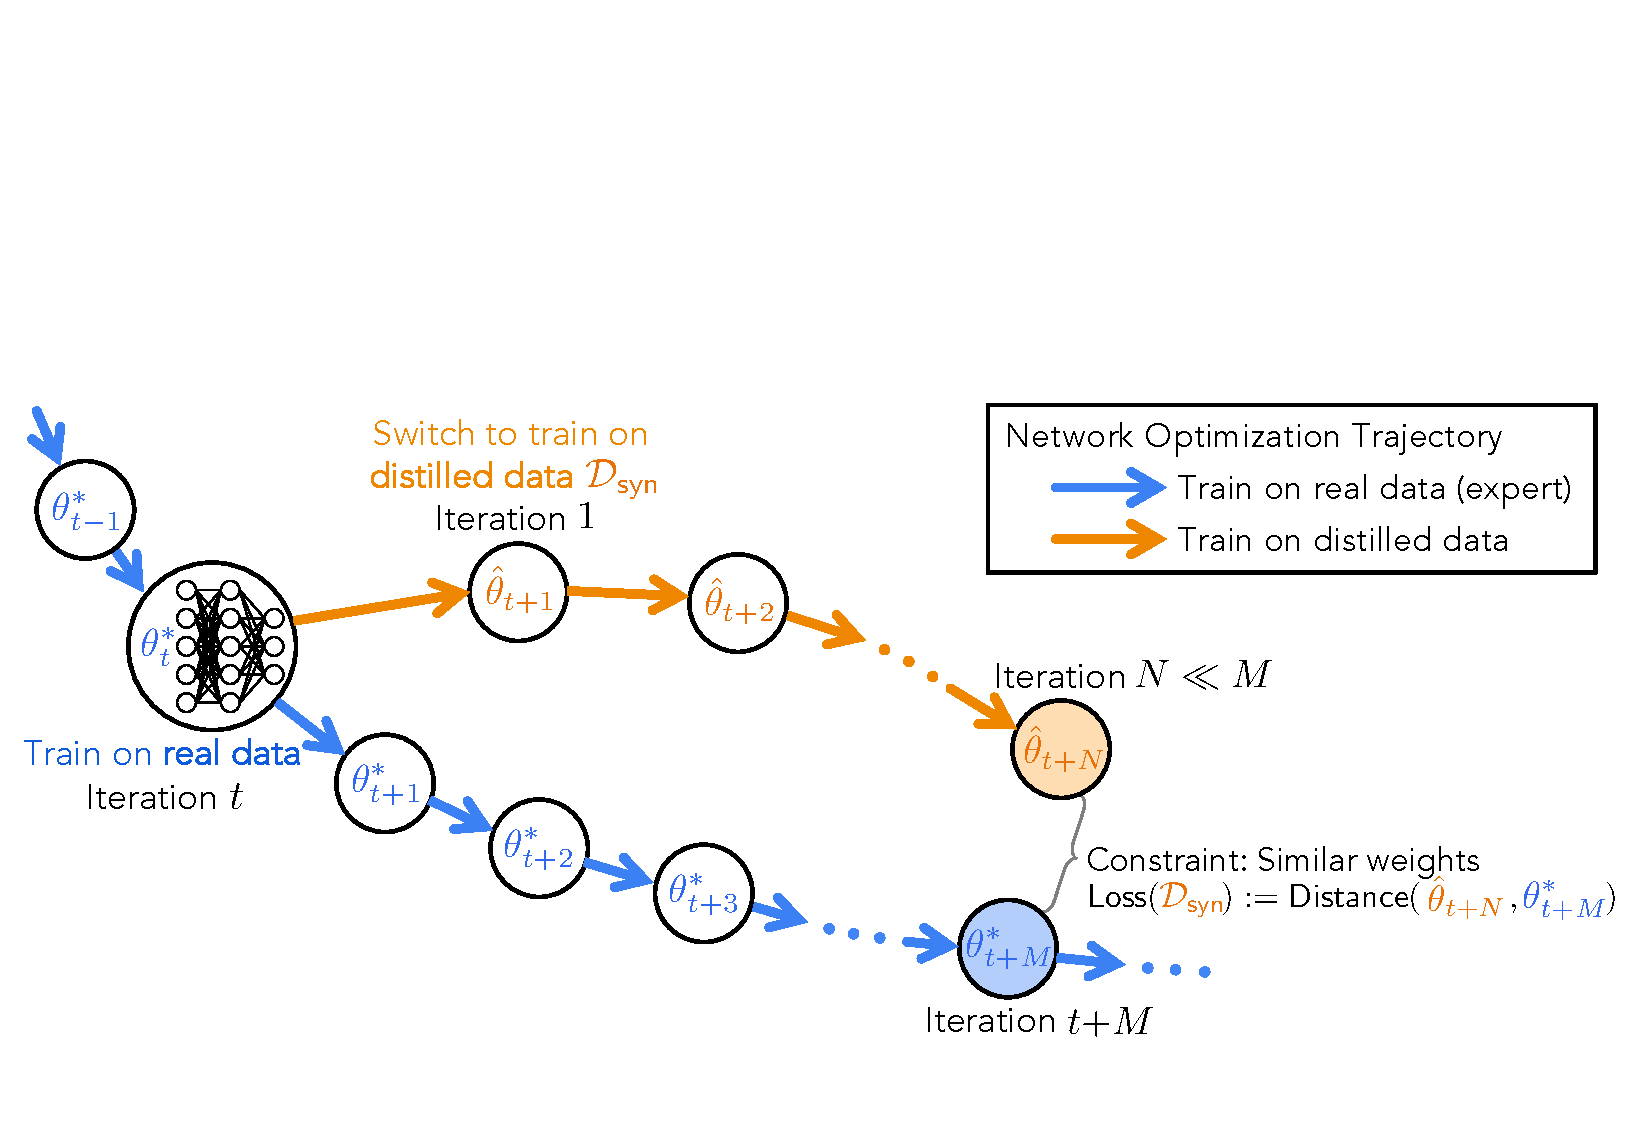
\includegraphics[scale=0.6, trim=0 42 0 190, clip]{figures/figure_3_our_method.pdf}\vspace{-0.18cm}
    \caption{We perform long-range parameter matching between training on distilled synthetic data and training on real data. Starting from the same initial parameters, we train distilled data $\mathcal{D}_\mathsf{syn}$ such that $N$ training steps on them match the same result (in parameter space) from much more $M$ steps on real data.}
    \lblfig{method_traj_match}
         \vspace{-6pt}
\end{figure*}


In our method, our loss function \textit{directly} encourages the distilled dataset to guide the network optimization along a similar trajectory (\Cref{fig:method_traj_match}). We first train a set of models from scratch on the real dataset and record their expert training trajectories. We then initialize a new model with a random time step from a randomly chosen expert trajectory and train for several iterations on the \textit{synthetic} dataset. Finally, we penalize the distilled data based on how far this synthetically trained network deviated from the expert trajectory and back-propagate through the training iterations. Essentially, we transfer the knowledge from many expert training trajectories to the distilled images. 

Extensive experiments show that our method handily outperforms existing dataset distillation methods as well as coreset selection methods on standard datasets, including CIFAR-10, CIFAR-100, and Tiny ImageNet. For example, we achieve 46.3\% with a \emph{single} image per class and 71.5\% with 50 images per class on CIFAR-10, compared to the previous state of the art (28.8\% / 63.0\% from \cite{dsa, dm} and 36.1\% / 46.5\% from \cite{nguyen2021dataset}).
Furthermore, our method also generalizes well to larger data, allowing us to see high $128\times128$-resolution images distilled from ImageNet \cite{deng2009imagenet} for the first time. Finally, we analyze our method through additional ablation studies and visualizations. %
\href{https://github.com/GeorgeCazenavette/mtt-distillation}{Code} and models are also available on our \href{https://georgecazenavette.github.io/mtt-distillation/}{webpage}.
\lblfig{intro}